 The case study presented in this paper was held at an exhibition with two main objectives:
\begin{enumerate}
	\item Cross-validate the findings obtained from a previous experiment~\cite{Angel2017-2}. This experiment was done to study the attribution of different linear and angular velocities, oscillation angle, direction, and orientation of the platform to \textit{Anger}, \textit{Happiness}, \textit{Sadness} and \textit{Fear}. A total of 196 value combinations were designed, 20 of which were presented to each participant. Subjects had to select for each presentation the most representative term describing it among the four emotions and two mental states (i.e., \textit{Excitement} and \textit{Tenderness}).
	\item Verify whether participants would prefer scenes when the robot moves expressing emotions or rather moves on the same trajectory without any emotion expression. To control scene variability two cameras and eight AR tags were used together with a Kalman filter to improve robot localization on the stage. AR tags were detected using the ROS package ar\_track\_alvar~\cite{artag2015}. The distribution of thecameras and the tags is reported in Figure~\ref{fig:setup_fourth}. 

\begin{figure}
	\centering
	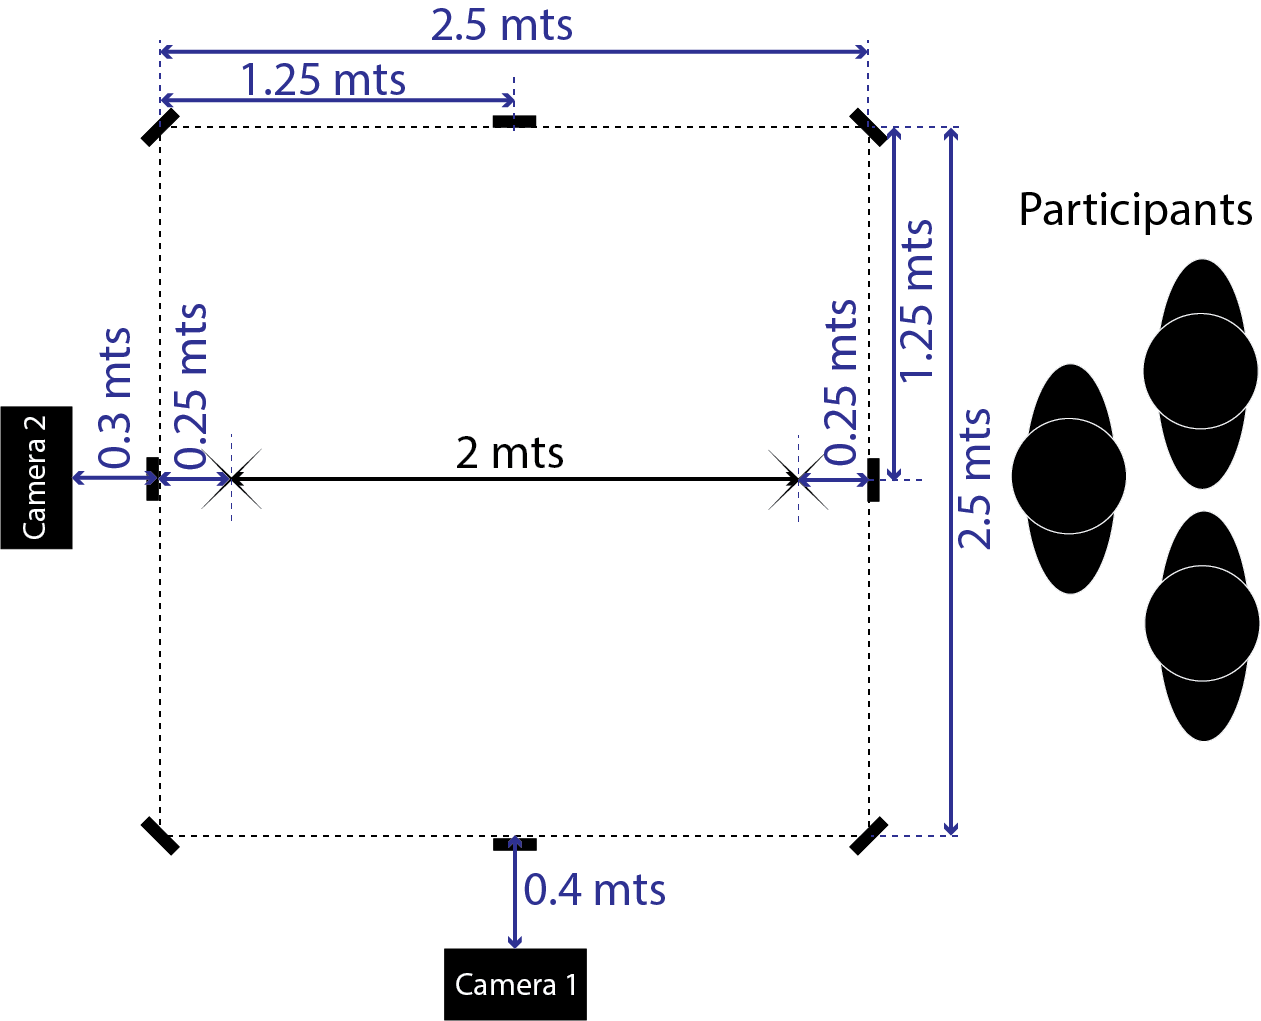
\includegraphics[width=0.45\textwidth]{./Images/FourthCase.png} 
	\caption{Environment setup for the case study. The crosses represent the starting points.}
	\label{fig:setup_fourth}
\end{figure}
 
\end{enumerate}

\subsection{Emotion Description}

The parameters selected to implement \textit{Anger}, \textit{Happiness}, \textit{Sadness} and \textit{Fear} are shown in Table~\ref{table:selected_fourth}. As it could be observed, two configurations for each emotion were selected among the ones evaluated in the previous experiment to be cross-checked. These configurations had to satisfy two conditions: (i) the linear velocity should be greater than $0$, so the robot should show some displacement, and (ii) it should be in the top 10 list of the configurations tested in the previous experiment.

\begin{table}
\centering
\small
\caption{Parameter values selected from the previous experiment.}
		\label{table:selected_fourth}
		\begin{tabular}{|c|p{0.9 cm}|p{0.9 cm}|p{0.9 cm}|p{1.05 cm}|p{0.9 cm}|}
			\hline
%\rotatebox{90}{\textbf{Emotion } }&
%\rotatebox{90}{\textbf{Direction  ($rad$)}}&
%\rotatebox{90}{\textbf{Orientation ($rad$)} }&
%\rotatebox{90}{\textbf{Linear Velocity ($mm/s$) }}&
%\rotatebox{90}{\textbf{Angular Velocity ($rad/s$) }}&
%\rotatebox{90}{\textbf{Angle ($rad$)}}\\	
\textbf{Emotion}&\textbf{Direc-tion  ($rad$)} & \textbf{Orien-tation ($rad$)} & \textbf{Linear Velocity ($mm/s$) } & \textbf{Angular Velocity ($rad/s$) } & \textbf{Angle ($rad$)} \\
			\hline
			Happiness-1&$0$&$0$&$500$&$3$&$0.349$\\
			\hline
			\co Happiness-2&\co $0$&\co $0$&\co $900$&\co $3$&\co $0.174$\\
			\hline
			Anger-1&$\pi$&$0$&$500$&$3$&$0.087$\\
			\hline
			\co Anger-2&\co $0$&\co $0$&\co $900$&\co $1$&\co $0.087$\\
			\hline
			Fear-1&$\pi$&$\pi$&$900$&$2$&$0.174$\\
			\hline
			\co Fear-2&\co $\pi$&\co $\pi$&\co $500$&\co $2$&\co $0.087$\\
			\hline
			Sadness-1&$\pi$&$0$&$200$&$1$&$0.349$\\
			\hline
			\co Sadness-2&\co $0$&\co $\pi$&\co $200$&\co $1$&\co $0.349$\\
			\hline
			\end{tabular}
\end{table}


\subsection{Scene}

Stage discretization was used to give zones of movements instead of absolute positions. This idea was brought from human theatrical actors, who arrange their movements based on zones on the stage~\cite{wilson2009theatre}. This allows them to adapt their position based on other actors and stage dimensions. The stage was discretized in 9x9 matrix as shown in Figure~\ref{fig:stage_division}. Robot's movements are given in terms of matrix positions to the Emotional Enrichment System. The robot's final position is calculated by the Emotional Enrichment System during execution. For instance, the scene was designedon a 3 x 3 meters stage, but in the presentation at teh exhibition the stage was 2.5 x 2.5 meters.

\begin{figure}
	\centering
	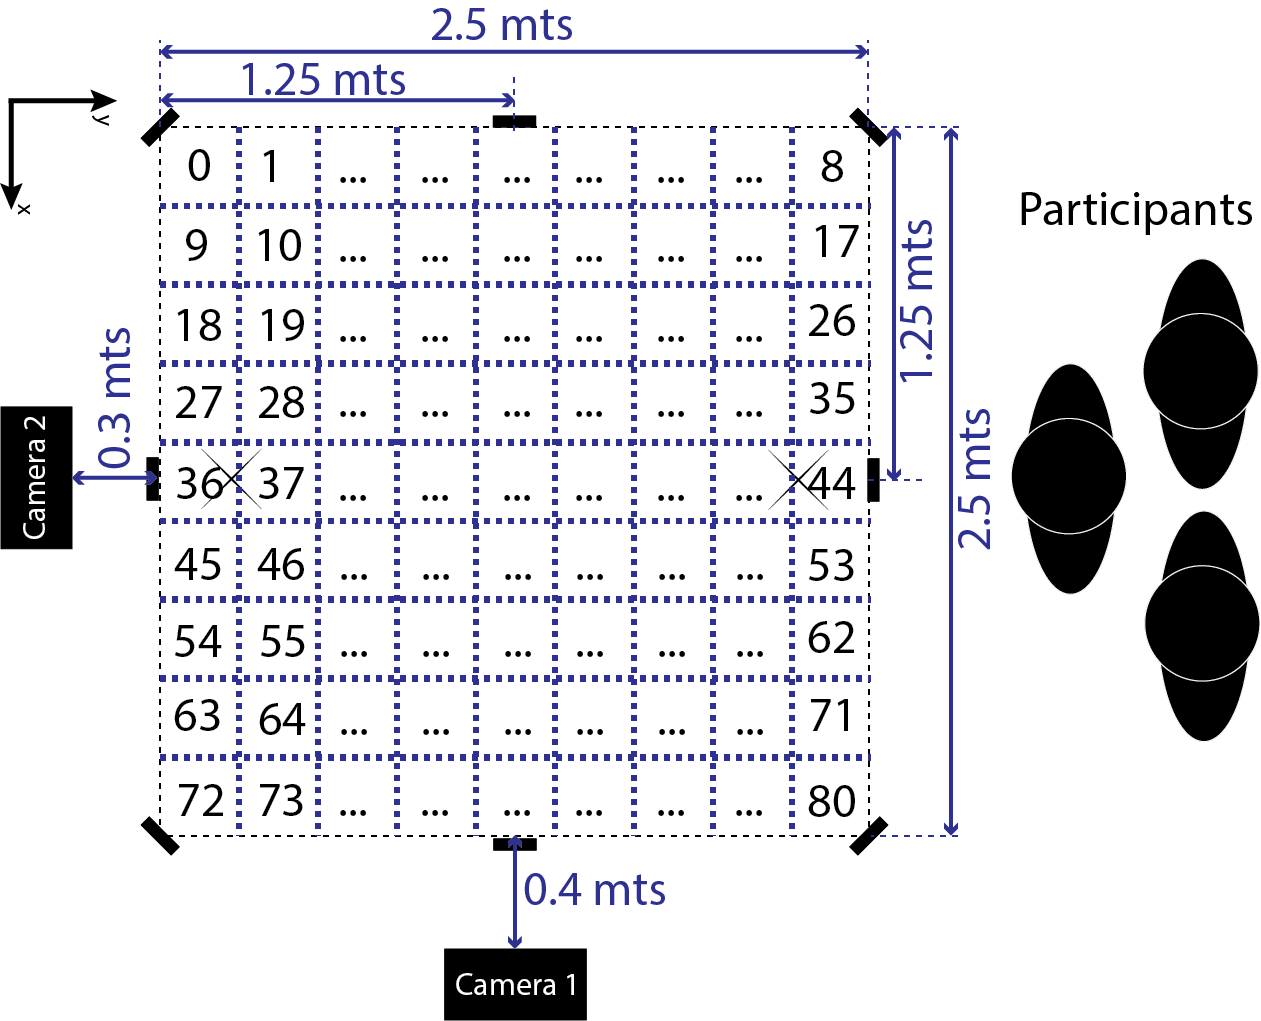
\includegraphics[width=0.45\textwidth]{./Images/FourthCaseScene.png} 
	\caption{Stage discretization  used for the scene. The blue squares correspond to the each zone, while the numbers correspond to the ID given to each zone.}
	\label{fig:stage_division}
\end{figure} 

The scene can be described as follows. The robot starts in the middle of the stage to move to the upstage right (See~\cite{Musical}), close to the right wing. Then, the robot moves to upstage right center and rotates to $\pi/2$ left (See~\cite{Artopia}). Next the robot moves to the right center. Then it goes to the center. When it arrives there, it turns full back and move backwards to downstage center with a full front orientation. There, it turns full back to move to center. Finally the robot turns to profile right and it does a step back; then it goes to the upstage center and then upstage right. The sequence of movements programmed to the robot are depicted in Figure~\ref{fig:movement}.
\begin{figure*}
	\centering
	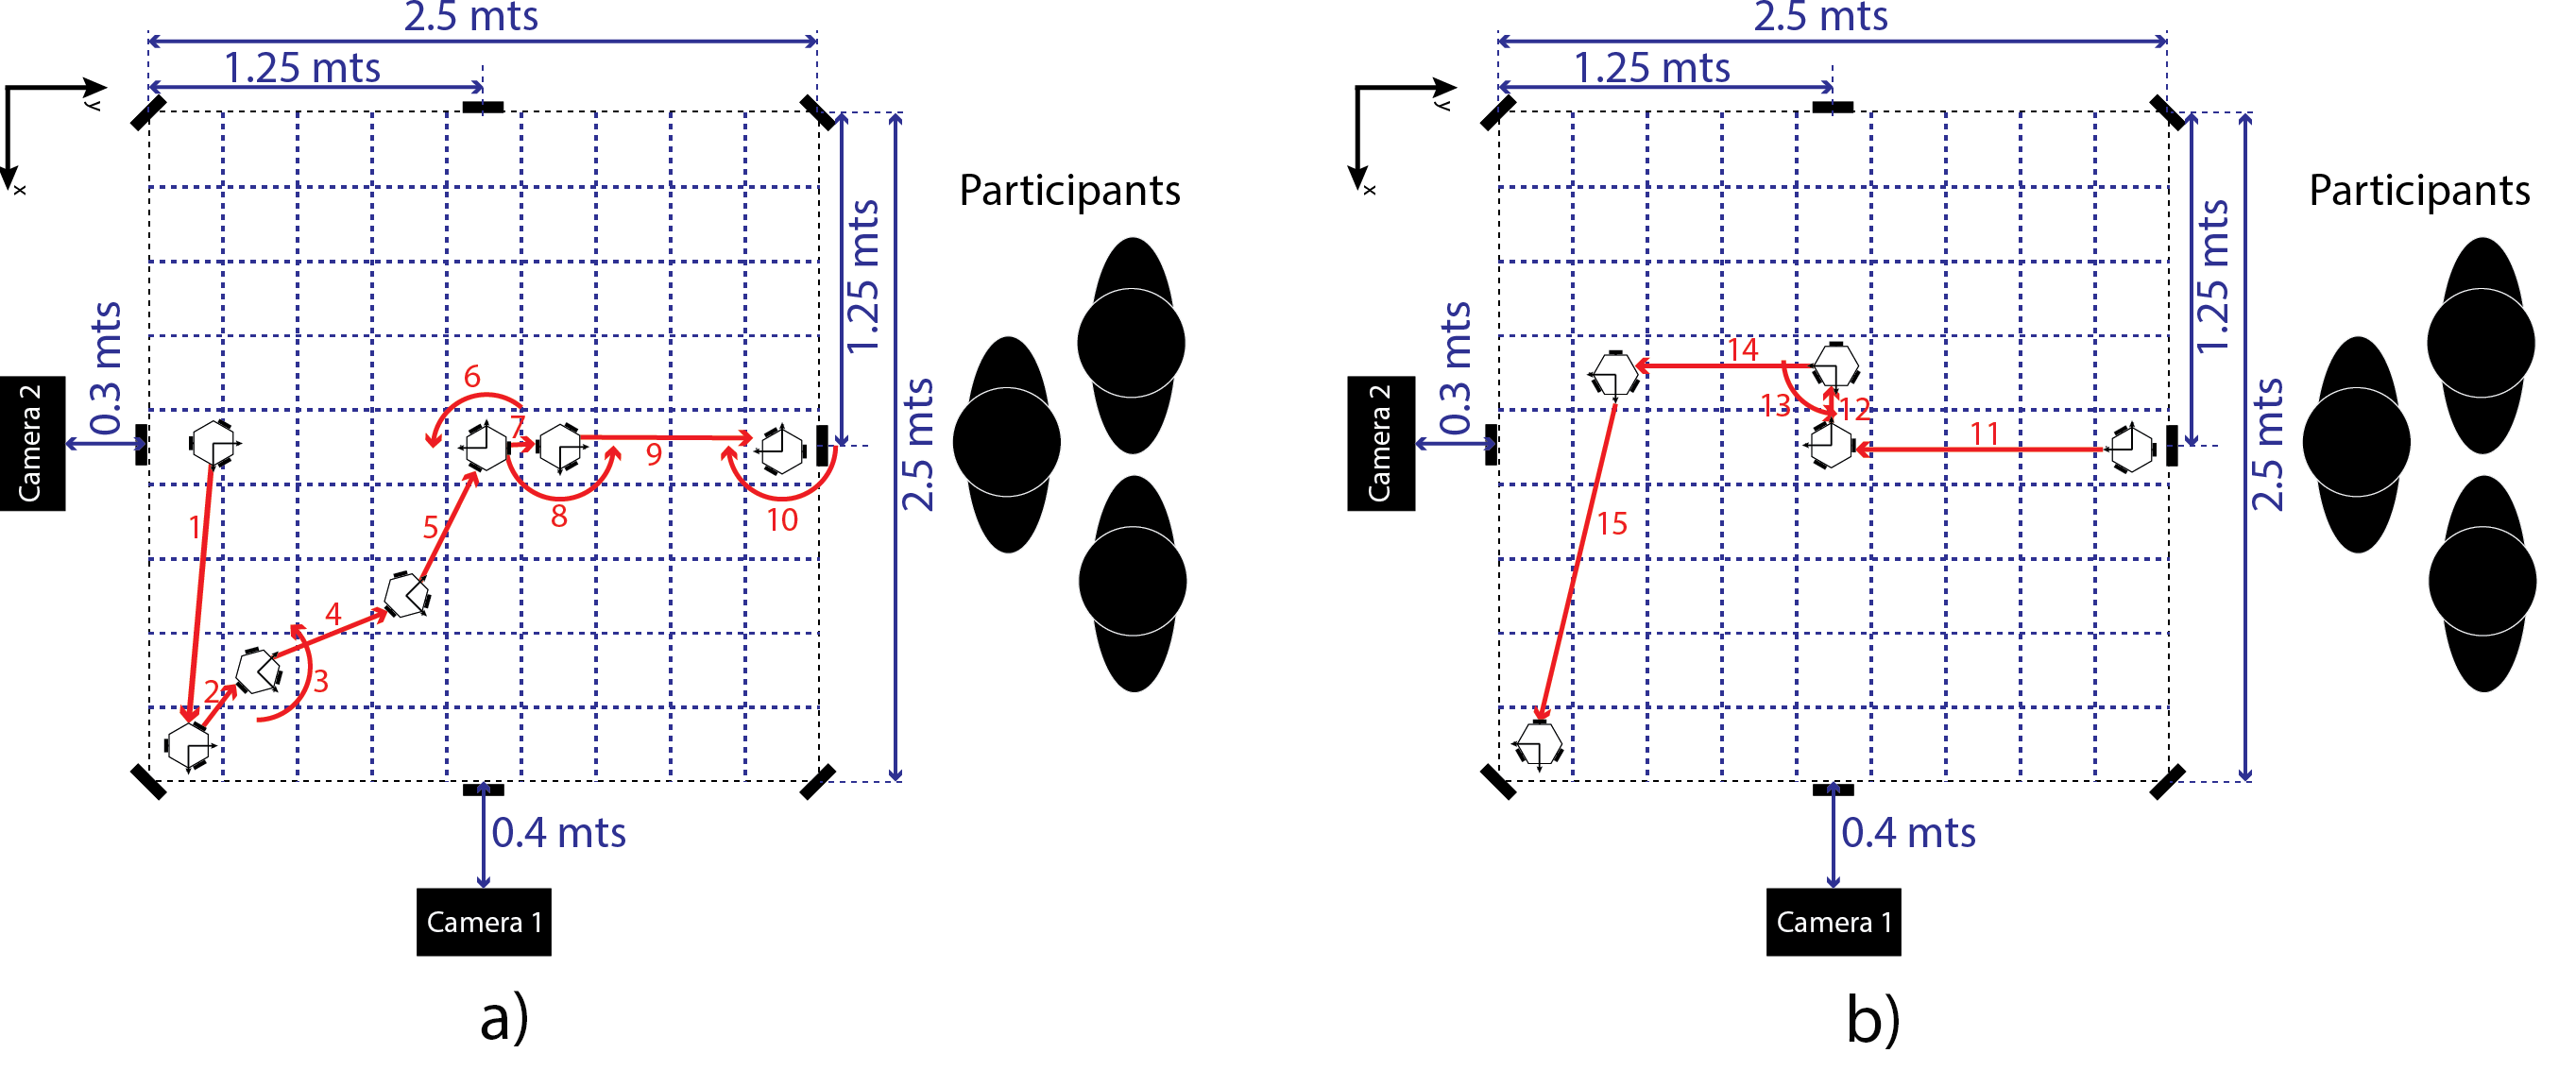
\includegraphics[width=0.95\textwidth]{./Images/fourthCaseSceneD.png} 
	\caption{Sequence of movements provided to the robot. The red arrows show the trajectory, while the numbers show the order among the movements. a) The first ten movements b) The last five movements }
	\label{fig:movement}
\end{figure*}

The relation between emotion and movement is as follow: movements one to five do not express any emotion. Movements six to ten show fear. Movement eleven depicts happiness, and the remaining movements depict sadness. The actions describing this scene are executed by the Emotional Enrichment System and the emotion selection is done manually via a graphical interface.

\subsection{Study}

This case study was done during Researchers' Night, 2015. During a period of two days, people were asked to participate in this study, which was divided in to parts. The first one, each subject was exposed to two rounds of emotions. The two emotions and their other were generated randomly before hand. The second part, participants were explained that a small scene was going to be presented twice. Thus, they should to selected the one they like more. The order of the scenes (e.g. with or without emotion) were generated beforehand. The total number of volunteers was 256: 128 males, 126 females, and 2 that chose not to specify their gender. The average age was 27.29 years, with standard deviation of 16.58, minimum age was 4 and maximum 76.
